\documentclass[11pt]{article}
\usepackage{tikz}
\usetikzlibrary{arrows.meta,positioning}
\usepackage{tabularx}
\usepackage{amsmath,amssymb,bm,graphicx,booktabs,hyperref,geometry}
\geometry{margin=1in}
\hypersetup{colorlinks=true, linkcolor=blue, citecolor=blue, urlcolor=blue}




\title{\textbf{Paper D-07: Financial Markets:\\ A Constraint-Driven Flux Dynamics (CDFD) Perspective}}
\author{Steve Bico Mujjabi, MD\\
\small Independent Researcher\\
\small Founder, Vura Labs\\
\small Kampala, Uganda\\
\small ORCID: 0009-0001-0556-5516}
\date{May 2026}


\newcommand{\EarthSuppPath}{Part\_A\_Earth\_Systems/supplementary/supplementary\_earth\_}
\newcommand{\EngSuppPath}{Part\_B\_Engineered\_Systems/supplementary/supplementary\_eng\_}
\newcommand{\SocSuppPath}{Part\_C\_Socioeconomic\_Systems/supplementary/supplementary\_soc\_}
\newcommand{\DomainSuppPath}{Part\_D\_Domain\_Applications/supplementary/supplementary\_dom\_}
\begin{document}

\maketitle
\newpage


\begin{abstract}
In this paper we apply Adaptive Flux Limitation (AFL) to financial market microstructure,
modelling order flow as constrained transport governed by the potential $\Phi = \Phi_{fundamental}
+ \Phi_{momentum} + \Phi_{sentiment}$ and constraint $C = C_{liquidity} + C_{balance-sheet} +
C_{regulatory}$. The AFL microstructure connects to macroeconomic AFL crises (Paper~33) via
the leverage-constraint erosion mechanism and the systemic cascade propagation criterion.

\textbf{Status: Inferred from AFL first principles; quantitative predictions are hypothesis-level.}\\
\textbf{Series tag: Dom-D07}
\end{abstract}

\section*{Symbol Conventions}

\noindent\textbf{CDFD/AFL Part IV symbol convention.}
\begin{center}
{\small
\begin{tabular}{p{0.15\linewidth}p{0.34\linewidth}p{0.41\linewidth}}
\hline
Symbol & Part IV meaning & Cross-domain reading \\
\hline
$\Phi$ & Driving flux or throughput & Energy, matter, signal, capital, information, traffic, force, or biological load entering a system \\
$C$ & Active constraint or capacity burden & Bottleneck, resistance, boundary, scarcity, toxicity, regulation, topology, latency, or load-bearing limit \\
$S$ & Responsiveness or adaptive surface & The system's ability to reconfigure, buffer, route, repair, learn, or preserve function under changing load \\
$M_s$ & Structural memory & Stored damage, hysteresis, inherited topology, institutional memory, trained weights, ecological legacy, or retained state \\
$\Psi_s$ & Adaptive operating ratio $(\Phi/C)\cdot S\cdot M_s$ & Local bookkeeping gauge for constrained operation, overload, recovery, or regime change; not a universal constant \\
$\Lambda$ & Life Number or capstone surplus ratio where explicitly defined & Reserved for Part II-derived life-number notation or synthesis-level surplus measures, never an undefined decoration \\
\hline
\end{tabular}
}
\end{center}

\noindent\textbf{Greek-symbol convention.}
\begin{center}
{\small
\begin{tabular}{p{0.15\linewidth}p{0.34\linewidth}p{0.41\linewidth}}
\hline
Symbol & Local role & Interpretation rule \\
\hline
$\alpha$ & Accumulation or reinforcement coefficient & Sets how fast a pathway, constraint, habit, cascade, or retained structure grows under load \\
$\beta$ & Relaxation, decay, clearance, or washout coefficient & Sets loss, recovery, damping, forgetting, degradation, or return toward baseline \\
$\gamma$ & Coupling, diffusion, redistribution, or transfer coefficient & Sets spread across nodes, layers, tissues, markets, infrastructures, media, or physical phases \\
$\delta,\epsilon$ & Perturbation, tolerance, small offset, or numerical guard & Used only as local thresholds, stability margins, measurement tolerances, or stress increments \\
$\eta,\lambda,\mu,\nu$ & Efficiency, rate, baseline, intensity, or frequency terms & Meaning is fixed by the equation, subscript, and domain-specific proxy in the paragraph where the term appears \\
$\rho,\sigma,\tau,\phi$ & Density/correlation, variability/noise, time-scale, phase, or field terms & Local coefficients only; subscripts bind them to the named pathway, domain, or experiment \\
$\Omega,\Lambda$ & Domain/state space; Life Number where defined & $\Omega$ names a modeled state space; $\Lambda$ carries life-number or synthesis notation only when the paper defines it \\
\hline
\end{tabular}
}
\end{center}


\section{Series Context}

Part I sets the flow--constraint language used here \cite{MujjabiPartI2026}. Part II develops the Life Number and the origins-of-life use of the same notation \cite{MujjabiPartII2026}. Part III applies AFL to biology and medicine \cite{MujjabiPartIII2026}. Part IV \cite{MujjabiPartIV2026}, DOI \url{https://doi.org/10.5281/zenodo.20395901}, is the cross-domain stress test: it asks where the notation clarifies measurement, and where it becomes only a metaphor.

\section{Introduction}


\subsection{The Mujjabi Universal Capacity Law}
Building directly upon the Fundamental Physics (Part I) \cite{MujjabiPartI2026}, the \textbf{Mujjabi Universal Capacity Law} proposes that across all scales---from black hole event horizons to global financial markets and power grids---driving high flux ($\Phi$) against a rigid topological constraint ($C$) can drive system saturation. When $\Phi/C$ approaches critical thresholds, the system does not scale linearly; it undergoes a topological phase transition.

\subsection{The Mujjabi Universal Memory Law}
The \textbf{Mujjabi Universal Memory Law} frames persistent systemic collapse. When a complex network fails to clear its structural memory ($M_s$) and its relaxation parameter decays ($\tau_{relax} \to \infty$), temporary stressors become permanent rigidities. This is the proposed CDFD mechanism behind ecological death, economic depressions, and infrastructural gridlock.


Global financial markets process $>10^9$ trades per day with total turnover exceeding \$100
trillion annually. High-frequency trading (HFT) algorithms operate on microsecond timescales,
submitting and cancelling millions of orders per second. This creates emergent AFL dynamics:
collective market behaviour arising from individual trader interactions, with stability properties
that cannot be predicted from individual trading strategies.

The financial AFL system exhibits canonical flux--constraint dynamics:
\begin{itemize}
    \item \textbf{Normal operation}: order flow matched to liquidity; prices efficiently incorporate
          information; $\Psi_s^* \approx 1$;
    \item \textbf{Stress}: declining liquidity ($C \downarrow$) as dealers reduce exposure; rising
          bid-ask spreads; $\Psi_s^* \to 1.2$;
    \item \textbf{Flash crash}: liquidity providers simultaneous withdrawal ($C \to C_{floor}$);
          $\Psi_s^* \to \infty$; cascade selling; prices move 5--20\% in seconds.
\end{itemize}

The AFL financial microstructure framework connects to the macroeconomic AFL crises of Paper~33:
microstructure $\Psi_s^*$ excursions are the market-level manifestation of the pre-crisis $C$
erosion and phase transition identified at the aggregate level. Financial systems also connect
to trade networks (Paper~27) through exchange rate dynamics and to governance (Paper~31) through
regulatory constraint modulation.

\section{Core Hypothesis}

\begin{center}
\textit{
Financial markets are AFL systems where order flow flux $\Phi$ is constrained by liquidity
$C$: efficient markets correspond to $\Psi_s^* \approx 1$ (order flow matched to market depth),
flash crashes are AFL constraint collapses ($C \to C_{floor}$, $\Psi_s^* \to \infty$), and
systemic crises are the macroeconomic AFL cascade triggered when financial microstructure
$\Psi_s^* > 1.2$ propagates to aggregate credit and institutional trust constraints.
}
\end{center}

AFL financial hypothesis: the Kyle (1985) market microstructure model --- where informed traders
face liquidity constraint from market makers --- is the AFL special case of financial microstructure.
The Kyle lambda (price impact of order flow) is the AFL $1/C$ parameter: high lambda (illiquid
market) = high $C^{-1}$ = low $C$. Efficient markets ($\lambda$ small, $C$ large) have $\Psi_s^*
\approx 1$; illiquid markets ($\lambda$ large, $C$ small) have $\Psi_s^* \gg 1$.
\textbf{Status: Hypothesis; Kyle-AFL mapping is analytic; empirical calibration requires
limit-order-book data.}

\section{Market Potential Fields}

We define the generalised market potential:
\begin{equation}
\Phi = \Phi_{fund} + \Phi_{mom} + \Phi_{sent}
\end{equation}
where:
\begin{itemize}
    \item $\Phi_{fund}$ --- fundamental value potential (discounted cash flows, earnings, book value;
          the primary long-run driver of equity prices; drives mean-reversion trading);
    \item $\Phi_{mom}$ --- momentum potential (price trend signal; drives trend-following algorithms
          and behavioral momentum traders; creates short-run correlation in returns);
    \item $\Phi_{sent}$ --- sentiment potential (retail investor mood, news flow, social media
          signal; highest-frequency, most volatile; amplifies $\Phi_{mom}$ in trending markets).
\end{itemize}

The gradient $\nabla\Phi$ represents the mispricing (distance from fundamental value): in
efficient markets, $\nabla\Phi_{fund}$ is rapidly eliminated by arbitrage (high $J_{arb}$);
in illiquid markets, $\nabla\Phi_{fund}$ persists because $C_{liquidity}$ prevents arbitrageurs
from trading sufficient size to close the gap.

\section{Market Liquidity as AFL Constraint}

\begin{equation}
C = C_{liquidity} + C_{balance-sheet} + C_{regulatory}
\end{equation}
where:
\begin{itemize}
    \item $C_{liquidity}$ --- market depth (number of shares/contracts available at bid and ask
          prices within 1--5\% of mid; the immediate trading constraint; measured by limit order
          book depth);
    \item $C_{balance-sheet}$ --- dealer balance sheet capacity (capital available to hold
          inventory and absorb order flow; regulated by Value-at-Risk and leverage limits;
          collapses in stress as dealers reduce gross exposure);
    \item $C_{regulatory}$ --- regulatory capital constraint (Basel III leverage ratio, Volcker
          Rule proprietary trading restrictions; raises structural floor of $C_{liquidity}$ but
          reduces $C_{balance-sheet}$ at the margin by constraining dealer risk-taking).
\end{itemize}

\subsection{Adaptive Surface Dynamics: Memory and Responsiveness}

The operating ratio $\Psi_s^*$ is mediated by adaptive surface components:
\begin{equation}
\Psi_s^* = (\Phi/C) \cdot S \cdot M_s
\end{equation}
where $S$ (Surface Responsiveness) and $M_s$ (Surface Memory) evolve as:
\begin{align}
\frac{dS}{dt} &= \kappa_s (\Psi_s^* - S) \\
\frac{dM_s}{dt} &= \Phi S - d_m M_s
\end{align}
These components represent the homeostatic capacity of the system to regulate its own operating ratio through memory and responsiveness.

\section{Flux Law}

Market order flow:
\begin{equation}
J_{order-flow} = -\frac{1}{C_{liquidity}}\nabla \Phi_{fund}
\end{equation}
where $\nabla\Phi_{fund}$ is the mispricing gradient (arbitrage opportunity) and $C_{liquidity}$
is market depth. This is the Almgren-Chriss optimal execution equation: order flow generates
price impact $1/C_{liquidity}$ per unit traded, which traders optimise against by spreading
execution over time.

\section{Conservation Dynamics}

Market price evolution:
\begin{equation}
\frac{\partial \Phi}{\partial t} = \nabla \cdot \left(\frac{1}{C}\nabla \Phi\right) + S
\end{equation}
where $S$ represents:
\begin{itemize}
    \item \textbf{Information arrival}: earnings releases, economic data, news events ($S > 0$
          for positive news, $S < 0$ for negative);
    \item \textbf{Central bank interventions}: quantitative easing raises $\Phi_{fund}$ by reducing
          discount rates;
    \item \textbf{Algorithmic order generation}: HFT strategies generate $\partial\Phi/\partial t$
          on microsecond timescales, amplifying volatility when $C_{liquidity}$ is low.
\end{itemize}

\section{Adaptive Constraint Dynamics}

Market liquidity evolves dynamically:
\begin{equation}
\frac{dC_{liquidity}}{dt} = \alpha_{liquidity}|J_{order-flow}| - \beta_{provision} C_{liquidity}
\end{equation}
where $\alpha_{liquidity}$ governs liquidity stress from order flow (large trades consume limit
order book depth; adverse selection risk reduces market-maker willingness to provide liquidity)
and $\beta_{provision}$ governs liquidity restoration (market makers replenish quotes after
trades; competition among liquidity providers restores depth between transactions).

Dealer balance sheet dynamics:
\begin{equation}
\frac{dC_{BS}}{dt} = -\alpha_{leverage}|J_{order-flow}| \cdot VaR_{shock} + \beta_{capital} C_{BS}.
\end{equation}

During stress: $VaR_{shock} \uparrow$ (rising volatility forces VaR limits) $\to C_{BS} \downarrow$
$\to C_{liquidity} \downarrow$ $\to$ $\Psi_s^* \uparrow$ $\to$ further volatility $\to$ positive
feedback.

\subsection{Adaptive Surface Dynamics: Memory and Responsiveness}

The operating ratio $\Psi_s^*$ is mediated by adaptive surface components:
\begin{equation}
\Psi_s^* = (\Phi/C) \cdot S \cdot M_s
\end{equation}
where $S$ (Surface Responsiveness) and $M_s$ (Surface Memory) evolve as:
\begin{align}
\frac{dS}{dt} &= \kappa_s (\Psi_s^* - S) \\
\frac{dM_s}{dt} &= \Phi S - d_m M_s
\end{align}
These components represent the homeostatic capacity of the system to regulate its own operating ratio through memory and responsiveness.

\section{Flux--Constraint Number and Market States}

\begin{equation}
\Psi_{s,market} = \frac{J_{order-flow}}{C_{liquidity} + C_{balance-sheet} + C_{regulatory}}
\end{equation}

\subsection{Normal Markets ($\Psi_s^* < 0.8$)}

Order flow well below liquidity capacity. Tight bid-ask spreads; deep limit order books; low
price impact. AFL predicts efficient price discovery: $\nabla\Phi_{fund}$ is rapidly arbitraged.
Volatility Index (VIX) $< 15$ correlates with $\Psi_s^* < 0.8$.

\subsection{Stressed Markets ($\Psi_s^* \approx 1$)}

Order flow approaches liquidity capacity. Widening bid-ask spreads; rising price impact; dealers
reducing inventory. AFL predicts critical slowing down: recovery from price shocks takes longer;
bid-ask autocorrelation rises. VIX 20--30 corresponds to $\Psi_s^* \approx 1$.

\subsection{Flash Crash / Liquidity Crisis ($\Psi_s^* > 1.2$)}

Order flow exceeds available liquidity. Market makers withdraw quotes ($C_{liquidity} \to
C_{floor}$); sell orders receive no bids; prices cascade. The AFL liquidity crisis criterion:
\begin{equation}
\frac{dC_{liquidity}}{dt} < -\alpha_{panic} \cdot C_{liquidity}, \quad \alpha_{panic} \gg \beta_{provision}.
\end{equation}

2010 Flash Crash AFL analysis: at 14:32 ET on May 6, 2010, a single algorithm submitted
\$4.1 billion in E-mini S\&P futures sell orders at a rate that consumed market depth faster
than $\beta_{provision}$ could restore it. $C_{liquidity} \to C_{floor}$ within 4 minutes;
$\Psi_{s,market} \to \infty$; cascade selling drove the Dow Jones down 1,000 points in 10 minutes.
Partial recovery occurred as liquidity providers returned ($\beta_{provision}$ restoring $C$).

\section{Market Microstructure and Information}

AFL derives the bid-ask spread from constraint dynamics:
\begin{equation}
\text{Spread} = \frac{2}{C_{liquidity}} \cdot |\nabla\Phi_{fund}|_{adverse-selection},
\end{equation}
where $|\nabla\Phi_{fund}|_{adverse-selection}$ is the expected mispricing from informed trader
orders. Market makers set $C_{liquidity}$ (quote size) to balance order flow capture against
adverse selection cost --- the AFL market-making optimisation.

Kyle's lambda (price impact per unit of order flow):
\begin{equation}
\lambda_{Kyle} = \frac{1}{2C_{liquidity}}.
\end{equation}

AFL predicts: $\lambda_{Kyle}$ rises (liquidity falls) as:
\begin{enumerate}
    \item volatility rises (adverse selection risk increases);
    \item concentration of informed traders increases (higher $\nabla\Phi_{fund}$ expected);
    \item dealer balance sheet declines (regulatory constraint tightens $C_{balance-sheet}$).
\end{enumerate}

\section{High-Frequency Trading as AFL Dynamics}

HFT algorithms operate in the millisecond AFL regime, creating dynamics invisible at slower
timescales:
\begin{itemize}
    \item \textbf{Market making HFT}: continuously restores $C_{liquidity}$ ($\beta_{provision}$
          large at ms scale); reduces $\Psi_{s,market}$ in normal conditions; withdraws in stress,
          making $C_{liquidity}$ collapse faster;
    \item \textbf{Statistical arbitrage HFT}: exploits $\nabla\Phi_{fund}$ at microsecond scale;
          AFL: high-frequency AFL routing along steepest gradient;
    \item \textbf{Momentum HFT}: amplifies $\Phi_{mom}$; raises $\Psi_{s,market}$ in trending
          markets; can trigger cascade when $\Psi_s^* > 1.2$.
\end{itemize}

HFT fragility: HFT market makers have $\beta_{provision}$ large but $C_{balance-sheet}$ small
(they hold minimal overnight inventory). In the AFL framework, small $C_{balance-sheet}$ means
the system operates at $\Psi_s^*$ close to 1 even in normal conditions --- providing the highest
efficiency but the smallest margin before cascade. AFL explains why post-2010 equity markets
have lower average bid-ask spreads but more frequent flash events.

\section{Pre-Crisis $\Psi_s^*$ Accumulation and Connection to Macro Crises}

Financial microstructure $\Psi_s^*$ connects to the macroeconomic AFL crisis framework (Paper~33):
\begin{equation}
\Psi_{s,macro-crisis} = f\left(\Psi_{s,microstructure}, \Psi_{s,credit}, \Psi_{s,institutional}\right).
\end{equation}

Pre-crisis accumulation dynamics (2006--2008):
\begin{enumerate}
    \item Low VIX ($\Psi_{s,microstructure} < 0.8$) induces dealer risk-taking; $C_{balance-sheet}$
          grows as leverage increases;
    \item Leverage ratio: $C_{balance-sheet}^{-1}$ rises from 15:1 (2003) to 30:1 (2007) as
          securitisation reduces apparent risk;
    \item Effective $C_{macro} \to C_{macro}/2$; $\Psi_{s,credit} \to 2\Psi_{s,credit,2003}$;
    \item Lehman Brothers failure (September 2008): $C_{interbank} \to C_{floor} \approx 0$;
          $\Psi_{s,interbank} \to \infty$; cascade to credit, equity, and FX markets simultaneously.
\end{enumerate}

AFL connection: market microstructure $\Psi_s^*$ is the highest-frequency indicator of the aggregate
AFL crisis that Paper~33 models at quarterly/annual timescales. Intraday $\Psi_s^*$ spikes are
the leading indicator of the multi-month $\Psi_s^*$ accumulation that precedes macro crises.

\section{Regulatory Constraint as AFL Policy}

Financial regulation is AFL constraint management:
\begin{itemize}
    \item \textbf{Basel III capital ratios}: raise structural floor of $C_{balance-sheet}$;
          AFL predicts that higher capital requirements reduce average $\Psi_{s,market}$ but also
          reduce $J_{credit}$ (lending) at the margin;
    \item \textbf{Volcker Rule}: limits proprietary trading, reducing $C_{balance-sheet}$
          deployment; AFL predicts reduced market depth ($C_{liquidity}$) in stress, increasing
          flash crash risk while reducing systemic leverage;
    \item \textbf{Circuit breakers}: automatic halts when $\Psi_{s,market} > \Psi_{s,circuit-breaker}$;
          AFL: externally imposed $J = 0$ giving $\beta_{provision}$ time to restore $C_{liquidity}$;
    \item \textbf{Securities Transaction Tax (Tobin tax)}: raises effective $C_{regulatory}$ for
          all trades; AFL predicts reduced HFT liquidity provision but also reduced $\Phi_{mom}$
          momentum cascades.
\end{itemize}

\section{Currency and Sovereign Bond Markets}

AFL extends to currency and sovereign debt markets:
\begin{itemize}
    \item \textbf{Exchange rates}: $\Psi_{s,FX} = J_{capital-flows} / C_{reserve-constraint}$;
          currency crises are $\Psi_{s,FX} > 1.2$ when capital outflows exceed reserve capacity;
    \item \textbf{Sovereign bonds}: $\Psi_{s,sov} = J_{debt-issuance} / C_{fiscal-capacity}$;
          sovereign debt crises are AFL events where fiscal constraint is overwhelmed by debt
          service requirements (Greece 2012, Argentina 2001);
    \item \textbf{Contagion}: $\Psi_{s,country-i} > 1.2 \Rightarrow \Psi_{s,country-j}$ rises via
          capital flow redirection and sentiment cascade.
\end{itemize}

\section{Predictions}

\begin{enumerate}
    \item \textbf{Flash crash early warning}: $\Psi_{s,market}$ computed from bid-ask spread and
          order book depth should exceed 1.0 in the 60 minutes preceding flash crash events;
          AFL predicts rising autocorrelation of bid-ask spread (critical slowing down) as
          leading indicator;
    \item \textbf{Kyle lambda scaling}: $\lambda_{Kyle} \propto 1/C_{liquidity} \propto \sigma_{volatility}$
          in normal markets; AFL predicts super-linear rise in $\lambda$ as $\Psi_s^* \to 1.2$;
    \item \textbf{Regulatory capital tradeoff}: raising capital requirements from 8\% to 12\%
          reduces $\Psi_{s,macro} $ by 30--40\% but reduces $J_{credit}$ by 10--15\%; AFL predicts
          this tradeoff from the constraint-throughput relationship;
    \item \textbf{HFT market making exit threshold}: HFT market makers withdraw when expected
          adverse selection cost $> \alpha_{liquidity}^{-1}$; AFL predicts this threshold from
          $C_{balance-sheet}$ and VaR parameters;
    \item \textbf{Circuit breaker optimal design}: AFL predicts optimal circuit breaker threshold
          at $\Psi_s^* = 1.1$ (before cascade begins) rather than the current 5--7\% price-drop
          trigger (which activates after cascade has started).
\end{enumerate}

\textbf{Status: Predictions 1--2 supported by market microstructure literature; predictions 3--5
are AFL-derived policy hypotheses.}

\section{Computational Interpretation}

The companion script \texttt{supplementary\_dom\_07.py} implements AFL financial market dynamics:
\begin{itemize}
    \item limit order book AFL: $C_{liquidity}(t)$ with HFT market-making and $\alpha$-decay from
          large orders; $\Psi_{s,market}(t)$ at millisecond resolution;
    \item flash crash simulation: large sell order submitted; $C_{liquidity}$ depletion; cascade;
          circuit breaker comparison (threshold sensitivity);
    \item pre-crisis accumulation: leverage erosion of $C_{balance-sheet}$ from 2003--2008;
          $\Psi_{s,credit}(t)$; Lehman trigger;
    \item regulatory scenario: capital ratio sweep; $J_{credit}$ vs $\Psi_{s,macro}$ tradeoff curve;
    \item outputs: $\Psi_{s,market}$ time series, flash crash anatomy, pre-crisis $\Psi_s^*$ accumulation.
\end{itemize}

\section{Discussion}

AFL provides a unified framework for financial markets from microsecond microstructure to decadal
macroeconomic cycles. The same $\Psi_s^* > 1.2$ threshold that governs flash crashes at the
millisecond scale governs financial crises at the annual scale --- AFL scale invariance
(Paper~40) at work. Market microstructure ($C_{liquidity}$) and macroeconomic constraint
($C_{institutional}$) are connected through the dealer balance sheet: when $C_{BS}$ collapses,
both microstructure and macro liquidity freeze simultaneously.

The AFL financial framework also reveals that post-crisis regulation (Basel III, Volcker Rule)
has correctly raised structural $C$ floors but has done so at the cost of reduced $J_{credit}$
and $J_{liquidity}$ --- the AFL constraint-throughput tradeoff that all regulation must navigate.
Optimal financial regulation is AFL constraint calibration: sufficient $C$ to prevent $\Psi_s^* >
1.2$ cascade while maintaining $J$ near the throughput required for economic growth.



\section{Measurement Layer}

The first job in any domain is to choose proxies before drawing conclusions. $\Phi$ may be a rate of material, energy, information, capital, or signal flow. $C$ is the bottleneck that slows or redirects that flow. $S$ measures the system's ability to reconfigure under stress, and $M_s$ records the past load that still changes present behavior. A useful application gives those four terms observable definitions, a time scale, and a failure condition. If a standard domain model explains the same data more cleanly, the CDFD/AFL mapping should give way.

\subsection{Current Runtime Diagnostic: Universal Network Cascade}
The release-local discovery script keeps this paper tied to the current CDFD Runtime \cite{CDFDRuntime2026}, including RK4 field updates, surface dynamics, structural-memory diffusion, and a finite-value audit. In the 2026-06-04 runtime pass, the localized hub-drive stress test ended with hub $\Psi_s=5.21$, peak network $\Psi_s=5.21$, 21 nodes above $\Psi_s>1.5$, and 37 maximum memory-locked nodes. I treat those numbers as a runtime sanity check and as a target for later domain measurement, not as a substitute for field data.


% BEGIN PART IV MAJOR UNIVERSAL UPGRADE
\section{Major Universal Upgrade: Mechanism, Scale, and Tests}

\subsection{Observable Translation}

The paper-specific translation begins with an observable chain rather than a
verbal analogy. For Financial Markets, the proposed drive is orders, leverage, information, credit, and investor demand.
The active limitation is liquidity, market depth, capital, collateral, and network exposure. Responsiveness is carried by
price discovery, market making, hedging, intervention, and substitution, while retained state is represented by
positions, losses, expectations, rules, and crisis history. The outcome to explain is volatility, liquidity, contagion, price formation, and recovery.

\begin{table}[htbp]
\centering
\small
\caption{Operational CDFD/AFL map for Paper D-07.}
\begin{tabularx}{\textwidth}{|l|X|X|}
\hline
\textbf{Term} & \textbf{Paper-specific observable meaning} & \textbf{Measurement question} \\
\hline
$\Phi$ & orders, leverage, information, credit, and investor demand & What rate, load, gradient, or demand enters the focal system? \\
\hline
$C$ & liquidity, market depth, capital, collateral, and network exposure & Which measured bottleneck limits transfer, function, or recovery? \\
\hline
$S$ & price discovery, market making, hedging, intervention, and substitution & Which process changes effective capacity or reroutes the load? \\
\hline
$M_s$ & positions, losses, expectations, rules, and crisis history & Which retained state makes equal present loads produce different futures? \\
\hline
$Y$ & volatility, liquidity, contagion, price formation, and recovery & Which outcome is predicted out of sample, with uncertainty? \\
\hline
\end{tabularx}
\end{table}

\begin{figure}[htbp]
\centering
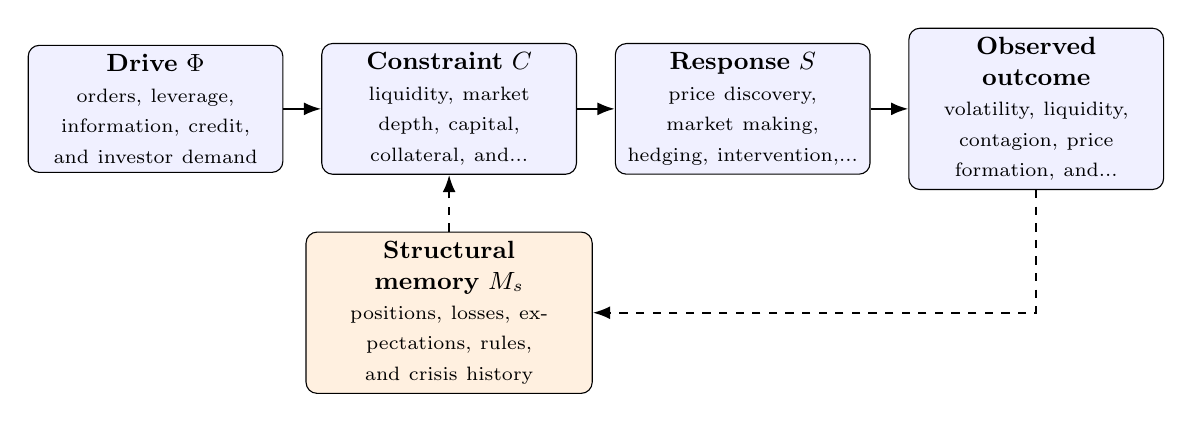
\begin{tikzpicture}[
    node distance=0.48cm,
    every node/.style={font=\small},
    box/.style={draw, rounded corners, align=center, minimum height=1.45cm, text width=3.0cm, fill=blue!6},
    memory/.style={draw, rounded corners, align=center, minimum height=1.25cm, text width=3.4cm, fill=orange!12},
    flow/.style={-{Latex[length=2.2mm]}, thick},
    feedback/.style={-{Latex[length=2.2mm]}, thick, dashed}
]
\node[box] (drive) {\textbf{Drive $\Phi$}\\\scriptsize orders, leverage, information, credit, and investor demand};
\node[box, right=of drive] (constraint) {\textbf{Constraint $C$}\\\scriptsize liquidity, market depth, capital, collateral, and...};
\node[box, right=of constraint] (response) {\textbf{Response $S$}\\\scriptsize price discovery, market making, hedging, intervention,...};
\node[box, right=of response] (outcome) {\textbf{Observed outcome}\\\scriptsize volatility, liquidity, contagion, price formation, and...};
\node[memory, below=0.72cm of constraint] (memory) {\textbf{Structural memory $M_s$}\\\scriptsize positions, losses, expectations, rules, and crisis history};
\draw[flow] (drive) -- (constraint);
\draw[flow] (constraint) -- (response);
\draw[flow] (response) -- (outcome);
\draw[feedback] (outcome.south) |- (memory.east);
\draw[feedback] (memory.north) -- (constraint.south);
\end{tikzpicture}
\caption{Paper D-07 observable CDFD/AFL architecture for Financial Markets. Solid arrows give the proposed forward chain; dashed arrows make history-dependent feedback explicit.}
\label{fig:d07-architecture}
\end{figure}

\subsection{Minimal Coupled Model}

A paper-level model must separate throughput, constraint accumulation, response,
and history. One deliberately minimal form is
\begin{align}
Y(t) &= \frac{\Phi(t)S(t)}{\epsilon + C(t)}, \\
\frac{dC}{dt} &= \alpha \Phi(t) - \beta S(t)C(t) + \gamma \mathcal{L}C(t), \\
\frac{dM_s}{dt} &= \eta C(t) - \mu M_s(t), \\
\Psi_s(t) &= \frac{\widehat{\Phi}(t)}{\epsilon+\widehat{C}(t)}\,
             \widehat{S}(t)\,[1+\omega\widehat{M_s}(t)] .
\end{align}
Here $Y$ is the measured output, $\epsilon>0$ prevents a singular denominator,
$\mathcal{L}$ is a spatial or network coupling operator, and hats denote
explicitly normalized variables. The sign and magnitude of $\omega$ must be
estimated: memory can preserve useful organization or amplify damage. No fixed
threshold is universal before the variables, normalization, and observation
scale are declared.

For this paper, the hypothesized causal sequence is specific. A change in
orders, leverage, information, credit, and investor demand arrives faster than price discovery, market making, hedging, intervention, and substitution can compensate.
This raises or redistributes liquidity, market depth, capital, collateral, and network exposure. If the load persists,
the retained state encoded by positions, losses, expectations, rules, and crisis history changes the next response, so a later event of equal
magnitude can produce a different trajectory in volatility, liquidity, contagion, price formation, and recovery. The
scientific task is to estimate that sequence against the best ordinary model of
the domain, not merely to redescribe the outcome after it occurs.

\subsection{Cross-Scale Universality Without Mechanistic Erasure}

For the domain applications family, the universal comparison is a disciplined translation test across systems with very different material mechanisms. A valid mapping preserves the baseline science of the domain, declares the scale of every variable, and earns its place through a discriminating prediction rather than resemblance alone. \cite{Holling1973,Turing1952,Shannon1948,BakTangWiesenfeld1987}
The CDFD programme is cumulative: Part I supplies the flow--constraint
foundation \cite{MujjabiPartI2026}; Part II asks when maintained throughput
supports persistent organized states \cite{MujjabiPartII2026}; Part III
develops adaptive limitation and biological memory \cite{MujjabiPartIII2026};
and Part IV \cite{MujjabiPartIV2026} tests how much of that architecture
survives translation. The CDFD Runtime \cite{CDFDRuntime2026} supplies a
reproducible numerical stress surface, but it does not substitute for the
domain evidence named here.

The required scale declaration for this paper is microseconds to decades; venues to global markets. At short
scales, the key question is whether the incoming drive is transmitted,
buffered, or diverted. At intermediate scales, response changes effective
capacity and network exposure. At long scales, retained structure can alter the
state space itself. A result is genuinely cross-scale only when the aggregation
rule is stated and the same conclusion is not an artifact of averaging.

\subsection{Evidence Ladder and Discriminating Tests}

\begin{table}[htbp]
\centering
\small
\caption{Evidence ladder for Paper D-07. Each rung can fail independently.}
\begin{tabularx}{\textwidth}{|p{0.17\textwidth}|X|X|}
\hline
\textbf{Test} & \textbf{Design} & \textbf{Discriminating result} \\
\hline
Proxy audit & Measure order books, trades, positions, funding data, networks, and interventions and preregister how each record maps to $\Phi$, $C$, $S$, $M_s$, and $Y$. & The mapping fails if proxies are non-identifiable, circular, or change meaning across cases. \\
\hline
Load ramp & Apply or observe a liquidity or information shock under contrasting leverage histories while estimating the dominant constraint and response time. & A threshold claim requires a reproducible nonlinear change and uncertainty bounds, not a visually chosen breakpoint. \\
\hline
Recovery and memory & Match present load across units with different histories, then compare recovery paths. & The memory claim requires history-dependent divergence after current conditions are controlled. \\
\hline
Model comparison & Compare the baseline domain model with and without the CDFD/AFL state variables using held-out data. & The paper's stated falsifier is: the mapping adds no value beyond established microstructure and risk models. \\
\hline
\end{tabularx}
\end{table}

The strongest practical design combines a prospective perturbation with a
recovery window. The load-ramp phase estimates where constraint begins to rise
faster than output. The recovery phase estimates $\beta$ and $\mu$, separating
fast relaxation from persistent memory. A topology or coupling intervention
then asks whether rerouting changes the cascade as predicted. Null results are
informative because they identify domains in which the universal notation adds
no measurable value.

\subsection{Research Programme and Boundary Conditions}

The immediate research programme has four steps. First, construct a documented
dataset from order books, trades, positions, funding data, networks, and interventions and retain raw units before normalization.
Second, fit a baseline domain model and report its calibration and out-of-sample
error. Third, add the smallest identifiable CDFD/AFL state extension and test
whether it improves prediction of volatility, liquidity, contagion, price formation, and recovery. Fourth, repeat the
analysis across the declared scale range and publish negative cases as part of
the universality audit.

Three boundaries are non-negotiable. Correlation between flow and failure does
not identify a constraint mechanism. A fitted memory term does not prove that
the stored state has the same material meaning in another domain. Finally, a
runtime cascade is evidence about the implementation, not evidence that the
real system follows it. The paper becomes stronger when it can say precisely
where the translation stops.


% END PART IV MAJOR UNIVERSAL UPGRADE

\section{Conclusion}

Financial markets are AFL systems across all timescales from microsecond HFT dynamics to
decadal macro cycles. Order flow, liquidity constraint, price discovery, flash crashes, and
systemic crises all emerge from the universal AFL equation with domain-appropriate $(\Phi, C)$
interpretation. AFL connects financial microstructure to all other Part~IV papers through the
universal flux--constraint framework.

\bibliographystyle{plain}
\bibliography{universal_afl_references}

\end{document}